\documentclass[12pt,a4paper]{article}
\usepackage{amsmath,amscd,amsbsy,amssymb,latexsym,url,bm,amsthm}
\usepackage{epsfig,graphicx,subfigure}
\usepackage{enumitem,balance}
\usepackage{wrapfig}
\usepackage{mathrsfs,euscript}
\usepackage[usenames]{xcolor}
\usepackage{hyperref}
\usepackage[vlined,ruled,linesnumbered]{algorithm2e}
\usepackage{array}
\hypersetup{colorlinks=true,linkcolor=black}
\usepackage{attachfile}
\usepackage{listings}
\usepackage{amsmath}
\usepackage{booktabs}
\usepackage{threeparttable}
\usepackage{graphicx} %插入图片的宏包
\usepackage{float} %设置图片浮动位置的宏包
\usepackage{subfigure} %插入多图时用子图显示的宏包
\usepackage{natbib}
\usepackage{amssymb,amsmath}
\usepackage{color}
\usepackage{multirow}

\newtheorem{theorem}{Theorem}
\newtheorem{lemma}[theorem]{Lemma}
\newtheorem{proposition}[theorem]{Proposition}
\newtheorem{corollary}[theorem]{Corollary}
\newtheorem{exercise}{Exercise}
\newtheorem*{solution}{Solution}
\newtheorem{definition}{Definition}
\theoremstyle{definition}

\renewcommand{\thefootnote}{\fnsymbol{footnote}}

\newcommand{\postscript}[2]
 {\setlength{\epsfxsize}{#2\hsize}
  \centerline{\epsfbox{#1}}}

\renewcommand{\baselinestretch}{1.0}

\setlength{\oddsidemargin}{-0.365in}
\setlength{\evensidemargin}{-0.365in}
\setlength{\topmargin}{-0.3in}
\setlength{\headheight}{0in}
\setlength{\headsep}{0in}
\setlength{\textheight}{10.1in}
\setlength{\textwidth}{7in}
\makeatletter \renewenvironment{proof}[1][Proof] {\par\pushQED{\qed}\normalfont\topsep6\p@\@plus6\p@\relax\trivlist\item[\hskip\labelsep\bfseries#1\@addpunct{.}]\ignorespaces}{\popQED\endtrivlist\@endpefalse} \makeatother
\makeatletter
\renewenvironment{solution}[1][Solution] {\par\pushQED{\qed}\normalfont\topsep6\p@\@plus6\p@\relax\trivlist\item[\hskip\labelsep\bfseries#1\@addpunct{.}]\ignorespaces}{\popQED\endtrivlist\@endpefalse} \makeatother

\begin{document}
\noindent

%========================================================================
\noindent\framebox[\linewidth]{\shortstack[c]{
\Large{\textbf{Lab06-Linear Programming}}\vspace{1mm}\\
CS214-Algorithm and Complexity, Xiaofeng Gao, Spring 2021.}}
\begin{center}
\footnotesize{\color{red}$*$ If there is any problem, please contact TA Haolin Zhou.}

% Please write down your name, student id and email.
\footnotesize{\color{blue}$*$ Name: Zirui Liu  \quad Student ID: 519021910343 \quad Email: L.prime@sjtu.edu.cn}
\end{center}

\begin{enumerate}
    \item
    \textit{Hirschberg Algorithm.} Recall the \textbf{String Similarity} problem in class, in which we calculate the edit distance between two strings in a sequence alignment manner.
    \begin{enumerate}
    	\item
    	Implement the algorithm combining \textbf{dynamic programming} and \textbf{divide-and-conquer} strategy in C/C++. Analyze the time complexity of your algorithm. {\color{blue}(The template \emph{Code-SequenceAlignment.cpp} is attached on the course webpage)}.
    	
    	\item
    	Given $\alpha(x, y) = |ascii(x) - acsii(y)|$, where $ascii(c)$ is the ASCII code of character $c$, and $\delta=13$. Find the edit distance between the following two strings.
    	\begin{align*}
    		X[1..60]=&\ CMQHZZRIQOQJOCFPRWOUXXCEMYSWUJ\\
    		&\ TAQBKAJIETSJPWUPMZLNLOMOZNLTLQ	
    	\end{align*}
    	\begin{align*}
    		Y[1..50]=&\ SUYLVMUSDROFBXUDCOHAATBKN\\
    		&\ AAENXEVWNLMYUQRPEOCJOCIMZ
    	\end{align*}
    \end{enumerate}
    \begin{solution}
    The results are here.\\
    \begin{figure}[H] %H为当前位置,!htb为忽略美学标准,htbp为浮动图形
    \centering %图片居中
    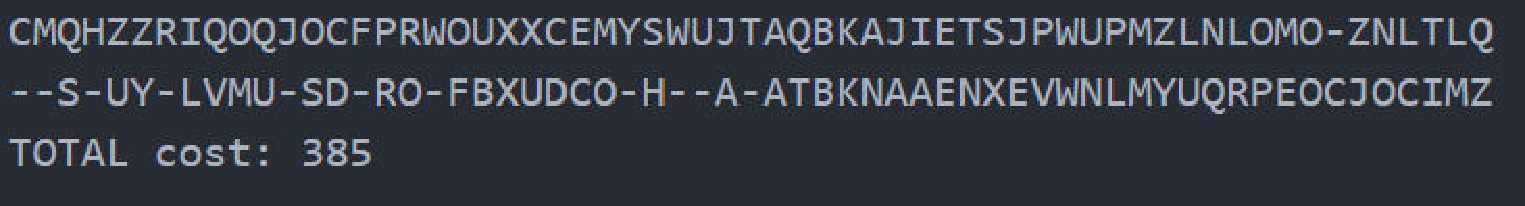
\includegraphics[width=0.5\textwidth]{result1.pdf}
     %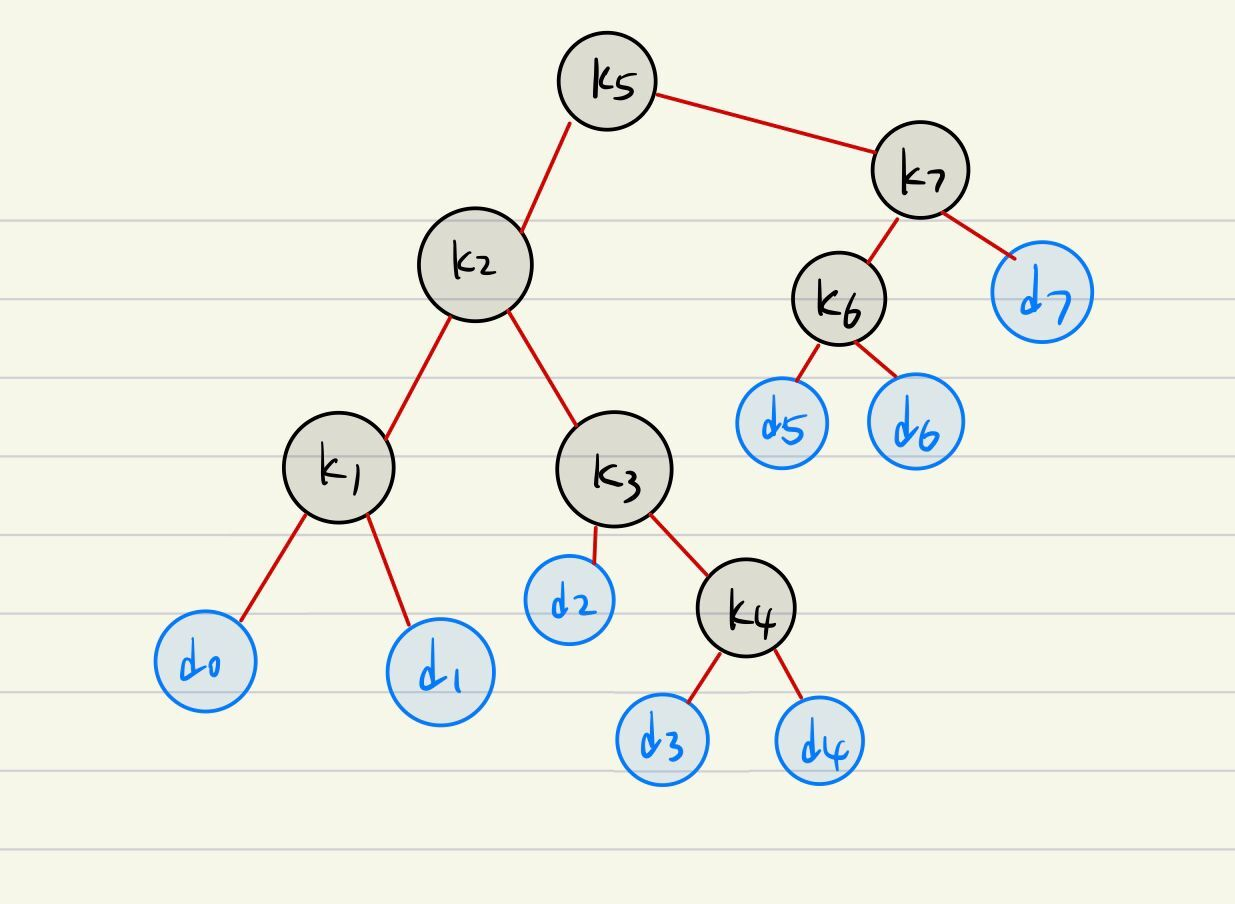
\includegraphics[width=1in]{tree.jpg}
    \caption{result1} %最终文档中希望显示的图片标题
    \label{} %用于文内引用的标签
    \end{figure}
    
    And codes can be found in the appendices.\\
    The time complexity is $O\left(mn\right)$.\\
    The time used to calculate a value for $Dp\left(s1,s2\right)$ is $O(|s1|*|s2|)$. Considering the recursion, The two top-leveled recursive calls each solve a smaller problem. Together these two sub-problems add up to half of the size of the original problem, which is $O\left(|s1|*{|s2|}/2\right)$ time complexity in total. Then we consider the next recursive level, which has four small sub-recursive problems in total, each one takes one quarter of the original size. Keep doing this, then we can conclude that the total time taken for the algorithm is $O\left(|s1|*|s2|*\left(1+1/2+1/4+...\right)\right)$ which is $O(2*|s1|*|s2|)$. That is $O(|s1|*|s2|)$. This use of recursion reduces the space used from O(|s1|*|s2|) to O(|s2|) and roughly doubles the time taken.
    
    
    \end{solution}
    
    \item 
    \textit{Travelling Salesman Problem.} Given a list of cities and the distances between each pair of cities ($ G=(V,E,W) $), we want to find the shortest possible route that visits each city exactly once and returns to the origin city. Similar to \textbf{Maximum Independent Set} and \textbf{Dominating Set}, please turn the traveling salesman problem into an ILP form.  
    
    \textbf{Remark:} $ W $ is the set of weights corresponds to the edges that connecting adjacent cities.  
    
    \begin{solution}
    Let us suppose that $x_{uv}$ be an indicator for whether there exists direct edge connecting two vertexes $u$ and $v$. $w_{uv}$ to be the weight of the directed edge from $u$ to $v$. $x_{uv}$ satisfies the following condition:\\
    $x_{uv}=$
    \begin{cases} 
    1,  & \mbox{if the salesman goes from $u$ to $v$ directly} \\
    0,  & \mbox{if the salesman doesn't go from $u$ to $v$ directly}
    \end{cases}\\
      Then we can transform the original problem to an $ILP$ problem. We want to have: $\sum_{u,v \in V} w_{uv}*x_{uv}$ having the least sum.
      
    
    \end{solution}
    
    
    
    
    \item
    \textit{Investment Strategy.} A company intends to invest $0.3$ million yuan in $2021$, with a proper combination of the following $3$ projects:
    \begin{itemize}
    \item \textbf{Project 1:} Invest at the beginning of a year, and can receive a $20\%$ profit of the investment in this project at the end of this year. Both the capital and profit can be invested at the beginning of next year;
    \item \textbf{Project 2:} Invest at the beginning of $2021$, and can receive a $50\%$ profit of the investment in this project at the end of $2022$. The investment in this project cannot exceed $0.15$ million dollars;
    \item \textbf{Project 3:} Invest at the beginning of $2022$, and can receive a $40\%$ profit of the investment in this project at the end of $2022$. The investment in this project cannot exceed $0.1$ million dollars.
    \end{itemize}
    Assume that the company will invest \emph{all} its money at the beginning of a year. Please design a scheme of investment in $2021$ and $2022$ which maximizes the overall sum of capital and profit at the end of $2022$.
    \begin{enumerate}
    \item
    Formulate a linear programming with necessary explanations.

    \item
    Transform your LP into its standard form and slack form.

    \item
    Transform your LP into its dual form.

    \item
    Use the simplex method to solve your LP.
    \end{enumerate}
    
    \begin{solution}
    (a):\\
    We assume that $x_1$ and $x_2$ separately to be investment for \textbf{Project 1} in year $2021$ and $2022$, $y$ and $z$ separately to be investment for \textbf{Project 2} and \textbf{Project 3}. The original problem can be transformed into the following linear programming problem: \\
    We want $max\left(1.2x_2+1.5y+1.4z\right)$\\
    And we have following conditions: \\
    $x_1+y = 0.3$\\
    $x_2+z = 1.2x_1$\\
    $y \leq 0.15$\\
    $z \leq 0.1$\\
    $x_1,x_2,y,z \ge 0$\\
    
    $Explanation: $\\    
    At the beginning of $2021$, we can only invest in Project 1 and Project 2 and since all the
    money must be used, we can get the equation $x_1 + y = 0.3$ holds.Then the money available can be invested at the beginning of 2022 is the profit from then end of 2021, which is clear that we can have  $x_2+z = 1.2x_1$.     $y \leq 0.15$, $z \leq 0.1$, $x_1,x_2,y,z \ge 0$ are basic requirements for \textbf{Project 2} and \textbf{Project 3}.
    
    (b):\\
    \textbf{Standard form: }\\
    We want $max\left(1.2x_2+1.5y+1.4z\right)$\\
    And we have following conditions: \\
    $x_1+y \leq 0.3$\\
    $x_2+z \leq 1.2x_1$\\
    $y \leq 0.15$\\
    $z \leq 0.1$\\
    $x_1,x_2,y,z \ge 0$\\
    
    \textbf{Slack form: }\\
    We want $max\left(1.2x_2+1.5y+1.4z\right)$\\
    We also assume $w_1$ and $w_2$ to be slack variables.\\
    And we have following conditions: \\
    $x_1+y = 0.3$\\
    $x_2+z = 1.2x_1$\\
    $y + w_1 = 0.15$\\
    $z + w_2 = 0.1$\\
    $x_1,x_2,y,z \ge 0$\\
    
    
    (c):\\
    \textbf{Dual form: }\\
    We want $min\left(0.3a_1-0.3a_2+0.15a_5+0.1a_6\right)$\\
    And we have following conditions: \\
    $a_1-a_2-1.2a_3+1.2a_4 \ge 0$\\
    $a_3-a_4 \ge 1.2$\\
    $a_1-a_2+a_5 \ge 1.5$\\
    $a_3-a_4+a_6 \ge 1.4$\\
    $a_1,a_2,a_3,a_4,a_5,a_6 \ge 0$\\
    
    
    
    (d):\\
    \textbf{Final solution: }\\
    
    $\Bar{x} = \left(0.15, 0.1, 0, 0\right)$\\
    We can solve that the result is 0.461.
    
    
    
    \end{solution}
    
    
    
    
    \item
    \textit{Factory Production.} An engineering factory makes seven products (PROD 1 to PROD 7) on the following machines: four grinders, two vertical drills, three horizontal drills, one borer and one planer. Each product yields a certain contribution to profit (in \pounds/unit). These quantities (in \pounds/unit) together with the unit production times (hours) required on each process are given below. A dash indicates that a product does not require a process.

    \begin{table}[htbp]
      \scriptsize
      \centering
      \renewcommand\arraystretch{1.1}
      \begin{tabular}{m{0.18\textwidth} m{0.07\textwidth}<{\centering} m{0.07\textwidth}<{\centering} m{0.07\textwidth}<{\centering} m{0.07\textwidth}<{\centering} m{0.07\textwidth}<{\centering} m{0.07\textwidth}<{\centering} m{0.07\textwidth}<{\centering}}
      \hline
       & \textbf{PROD 1} & \textbf{PROD 2} & \textbf{PROD 3} & \textbf{PROD 4} & \textbf{PROD 5} & \textbf{PROD 6} &  \textbf{PROD 7} \\\hline
      Contribution to profit & 10 & 6 & 8 & 4 & 11 & 9 & 3 \\
      Grinding & 0.5 & 0.7 & - & - & 0.3 & 0.2 & 0.5 \\
      Vertical drilling & 0.1 & 0.2 & - & 0.3 & - & 0.6 & - \\
      Horizontal drilling & 0.2 & - & 0.8 & - & - & - & 0.6 \\
      Boring & 0.05 & 0.03 & - & 0.07 & 0.1 & - & 0.08 \\
      Planing & - & - & 0.01 & - & 0.05 & - & 0.05 \\
      \hline
      \end{tabular}
    \end{table}

    There are marketing limitations on each product in each month, given in the following table:

    \begin{table}[htbp]
      \scriptsize
      \centering
      \renewcommand\arraystretch{1.1}
      \begin{tabular}{m{0.1\textwidth} m{0.07\textwidth}<{\centering} m{0.07\textwidth}<{\centering} m{0.07\textwidth}<{\centering} m{0.07\textwidth}<{\centering} m{0.07\textwidth}<{\centering} m{0.07\textwidth}<{\centering} m{0.07\textwidth}<{\centering}}
      \hline
       & \textbf{PROD 1} & \textbf{PROD 2} & \textbf{PROD 3} & \textbf{PROD 4} & \textbf{PROD 5} & \textbf{PROD 6} &  \textbf{PROD 7} \\\hline
      January & 500 & 1000 & 300 & 300 & 800 & 200 & 100 \\
      February & 600 & 500 & 200 & 0 & 400 & 300 & 150 \\
      March & 300 & 600 & 0 & 0 & 500 & 400 & 100 \\
      April & 200 & 300 & 400 & 500 & 200 & 0 & 100 \\
      May & 0 & 100 & 500 & 100 & 1000 & 300 & 0 \\
      June & 500 & 500 & 100 & 300 & 1100 & 500 & 60 \\
      \hline
      \end{tabular}
    \end{table}

    It is possible to store up to 100 of each product at a time at a cost of \pounds0.5 per unit per month (charged at the end of each month according to the amount held at that time). There are no stocks at present, but it is desired to have a stock of exactly 50 of each type of product at the end of June. The factory works six days a week with two shifts of 8h each day. It may be assumed that each month consists of only 24 working days. Each machine must be down for maintenance in one month of the six. No sequencing problems need to be considered.

    When and what should the factory make in order to maximize the total net profit?

    \begin{enumerate}
    \item
    Use \emph{CPLEX Optimization Studio} to solve this problem. Describe your model in \emph{Optimization Programming Language} (OPL). Remember to use a separate data file (.dat) rather than embedding the data into the model file (.mod).

    \item
    Solve your model and give the following results.
    \begin{enumerate}
    \item
    For each machine:
    \begin{enumerate}
    \item
    the month for maintenance.\\
    This can be checked out in the next chart, where the month for maintenance has zero amount to make.
    \end{enumerate}
    \item
    For each product:
    \begin{enumerate}
    \item
    The amount to make in each month.\\
    
     \begin{table}[htbp]
      \scriptsize
      \centering
      \renewcommand\arraystretch{1.1}
      \begin{tabular}{m{0.1\textwidth} m{0.07\textwidth}<{\centering} m{0.07\textwidth}<{\centering} m{0.07\textwidth}<{\centering} m{0.07\textwidth}<{\centering} m{0.07\textwidth}<{\centering} m{0.07\textwidth}<{\centering} m{0.07\textwidth}<{\centering}}
      \hline
       & \textbf{PROD 1} & \textbf{PROD 2} & \textbf{PROD 3} & \textbf{PROD 4} & \textbf{PROD 5} & \textbf{PROD 6} &  \textbf{PROD 7} \\\hline
    Jan	& 500.0	& 1000.0	& 300.0	& 300.0	& 800.0	& 200.0	& 100.0\\
    Feb	& 600.0	& 500.0	& 200.0	& 0.0	& 400.0	& 300.0	& 150.0\\
    Mar	& 400.0	& 700.0	& 100.0	& 100.0	& 600.0	& 400.0	& 200.0\\
    Apr	& 0.0	& 0.0	& 0.0	& 0.0	& 0.0	& 0.0	& 0.0\\
    May	& 0.0	& 100.0	& 500.0	& 100.0	& 1000.0	& 300.0	& 0.0\\
    Jun	& 550.0	& 550.0	& 150.0	& 350.0	& 1150.0	& 550.0	& 110.0\\

      \hline
      \end{tabular}
    \end{table}
    
    
    \item
    The amount to sell in each month.
    
         \begin{table}[htbp]
      \scriptsize
      \centering
      \renewcommand\arraystretch{1.1}
      \begin{tabular}{m{0.1\textwidth} m{0.07\textwidth}<{\centering} m{0.07\textwidth}<{\centering} m{0.07\textwidth}<{\centering} m{0.07\textwidth}<{\centering} m{0.07\textwidth}<{\centering} m{0.07\textwidth}<{\centering} m{0.07\textwidth}<{\centering}}
      \hline
       & \textbf{PROD 1} & \textbf{PROD 2} & \textbf{PROD 3} & \textbf{PROD 4} & \textbf{PROD 5} & \textbf{PROD 6} &  \textbf{PROD 7} \\\hline      
    Jan	& 500.0	& 1000.0	& 300.0	& 300.0	& 800.0	& 200.0	& 100.0\\
    Feb	& 600.0	& 500.0	& 200.0	& 0.0	& 400.0	& 300.0	& 150.0\\
    Mar	& 300.0	& 600.0	& 0.0	& 0.0	& 500.0	& 400.0	& 100.0\\
    Apr	& 100.0	& 100.0	& 100.0	& 100.0	& 100.0	& 0.0	& 100.0\\
    May	& 0.0	& 100.0	& 500.0	& 100.0	& 1000.0	& 300.0	& 0.0\\
    Jun	& 500.0	& 500.0	& 100.0	& 300.0	& 1100.0	& 500.0	& 60.0\\

      \hline
      \end{tabular}
    \end{table}
    
    \newpage

    \item
    The amount to hold at the end of each month.
    
    \begin{table}[htbp]
      \scriptsize
      \centering
      \renewcommand\arraystretch{1.1}
      \begin{tabular}{m{0.1\textwidth} m{0.07\textwidth}<{\centering} m{0.07\textwidth}<{\centering} m{0.07\textwidth}<{\centering} m{0.07\textwidth}<{\centering} m{0.07\textwidth}<{\centering} m{0.07\textwidth}<{\centering} m{0.07\textwidth}<{\centering}}
      \hline
       & \textbf{PROD 1} & \textbf{PROD 2} & \textbf{PROD 3} & \textbf{PROD 4} & \textbf{PROD 5} & \textbf{PROD 6} &  \textbf{PROD 7} \\\hline      
    Jan	& 0.0	& 0.0	& 0.0	& 0.0	& 0.0	& 0.0	& 0.0\\
    Feb	& 0.0	& 0.0	& 0.0	& 0.0	& 0.0	& 0.0	& 0.0\\
    Mar	& 100.0	& 100.0	& 100.0	& 100.0	& 100.0	& 0.0	& 100.0\\
    Apr	& 0.0	& 0.0	& 0.0	& 0.0	& 0.0	& 0.0	& 0.0\\
    May	& 0.0	& 0.0	& 0.0	& 0.0	& 0.0	& 0.0	& 0.0\\
    Jun	& 50.0	& 50.0	& 50.0	& 50.0	& 50.0	& 50.0	& 50.0\\

      \hline
      \end{tabular}
    \end{table}
    
    
    
    \end{enumerate}
    \item
    The total selling profit.\\
    $\$109330$
    \item
    The total holding cost.\\
    $\$475$
    
    \item
    The total net profit (selling profit minus holding cost).\\
    $\$108855.00$
    
    \end{enumerate}
    \end{enumerate}
    \textbf{Remark:} You can choose to use the attached .dat file or write it yourself. 

\end{enumerate}

\begin{solution}
For personal reasons that I have set-up Gurobi in MCM, so I used Gurobi instead of cplex. The codes can be seen in appendices.

\end{solution}

\newpage

\begin{appendices}
\section{First appendix: code-test.cpp}
\textcolor[rgb]{0.98,0.00,0.00}{\textbf{Input C++ source1:}}
\lstinputlisting[language=c++]{./code-test.cpp}

%\t

%\section{Second appendix}

%\textcolor[rgb]{0.98,0.00,0.00}{\textbf{Input python source2:}}
%\lstinputlisting[language=python]{./code/fire_data.py}

\end{appendices}

\newpage

\begin{appendices}
\section{Second appendix: gurobi.py}
\textcolor[rgb]{0.98,0.00,0.00}{\textbf{Input python source2:}}
\lstinputlisting[language=python]{./gurobi.py}

\end{appendices}

\newpage
\vspace{20pt}

{\noindent\large\textbf{Appendix}}
\begin{enumerate}
	\item [\textbf{A.}]
	\textbf{FactoryPlanning.dat}
	\attachfile{FactoryPlanning.dat}
	\lstset{
		language=C,
		tabsize=2,
		basicstyle=\footnotesize\ttfamily,
		columns=fullflexible,
		keywordstyle=\color{blue},
		numbers=left,
		numberstyle=\scriptsize\ttfamily,
		frame=single
	}
	\begin{lstlisting}
		NbMonths = 6;
		
		Prod = {Prod1, Prod2, Prod3, Prod4, Prod5, Prod6, Prod7};
		Process = {Grind, VDrill, HDrill, Bore, Plane};
		
		// profitProd[j] is profit per unit for product j
		ProfitProd = [10 6 8 4 11 9 3];
		
		// processProd[i][j] gives hours of process i required by product j
		ProcessProd = [[0.5  0.7  0.0  0.0  0.3  0.2 0.5 ]
		[0.1  0.2  0.0  0.3  0.0  0.6 0.0 ]
		[0.2  0.0  0.8  0.0  0.0  0.0 0.6 ]
		[0.05 0.03 0.0  0.07 0.1  0.0 0.08]
		[0.0  0.0  0.01 0.0  0.05 0.0 0.05]];
		
		// marketProd[i][j] gives marketing limitation on product j for month i
		MarketProd = [[500 1000 300  300 800  200 100]
		[600 500  200  0   400  300 150]
		[300 600  0    0   500  400 100]
		[200 300  400  500 200  0   100]
		[0   100  500  100 1000 300 0  ]
		[500 500  100  300 1100 500 60 ]];
		
		CostHold  = 0.5;
		StartHold = 0;
		EndHold   = 50;
		MaxHold   = 100;
		
		// process capacity
		HoursMonth = 384; // 2 eight hour shifts per day, 24 working days per month;
		
		// number of each type of machine
		NumProcess = [4 2 3 1 1];
		
		// how many machines must be down over 6 month period
		NumDown = [4 2 3 1 1];
	\end{lstlisting}
\end{enumerate}

\textbf{Remark:} You need to include your .cpp, .mod, .dat, .pdf and .tex files in your uploaded .zip file.

%========================================================================
\end{document}
